\documentclass[11pt, titlepage]{article}
\usepackage{epsfig,latexsym}
\usepackage{amsmath}
\usepackage{graphicx}
\usepackage{placeins}
\usepackage{fancyhdr}
\usepackage{listings}
\usepackage{gensymb}


\setlength{\textwidth}{7.25in}
\setlength{\textheight}{9.5in}
\setlength{\topmargin}{-0.75in}
\setlength{\oddsidemargin}{-0.5in}
\setlength{\evensidemargin}{-0.5in}
\setlength{\headheight}{26pt}

\lstset{
    basicstyle = \footnotesize,
    breakatwhitespace = false,
	breaklines = true,
	language = C,
	frame=single,
	tabsize=2
}

\pagestyle{fancy}
\fancyhead[R]{EEC 172 Lab4 \\
    			Richard Szeto \& Sean Ho}

\title{EEC 172 Lab4}

\author{Richard Szeto \& Sean Ho}

\date{Wednesday, March 6, 2013}

\begin{document}

    \maketitle
    
    \section{Objectives}
        \subsection{Part I}
            The objectives of part I is to generate two valid PWM signals in the LM3S2110 and be able to use the IR remote to alter the PWM signal within the legal bounds. The left and right buttons will control one of the PWM signals, and the up and down buttons will control the other PWM signal.
        \subsection{Part II}
            The objectives of part II is to use the PWM signals produced in part I to control the servo by using the IR remote to alter the PWM signal within the legal bounds. The left and right buttons will control the pan rotation, and the up and down buttons will control the tilt rotation.
        \subsection{Part III}
            The objectives of part III is to control the PWM signals in the LM3S2110 by using the IR remote to send XBee packets from the LM3S8962 to the LM3S2110. The packets sent will have values corresponding to the pan and tilt rotations.
    \section{Procedures}
        \subsection{Part I}
            We used the pwmgen code given in the Stellaris folder as a template. To accomodate for the LM3S2110, we changed the output ports of the PWM signal to PF0 and PF1. An mathematical calculation was used to produce two 1.5ms control pules with frequencies of 50Hz. After confirming that our control signals match these specification through the use of the logic analyzer, we incorporated Lab3's code to allow the use of the IR remote. An Algorithm was used to determine how much of the control signal would be changed each time the up, down, left, and right buttons are pressed. When the up/down buttons are pressed, the PWM signal on channel 1 will decrease/increase by 0.1ms. The PWM signal on channel 1 has an upper bound of 2.0ms and a lower bound of 1.0ms. When the left/right buttons are pressed, the PWM signal on channel 2 will decrease/increase by 0.05ms. The PWM signal on channel 2 has an upper bound of 2.0ms and a lower bound of 1.0ms.
        \subsection{Part II}
            We needed to convert the PWM pulse widths to map to the angles available to the servo. The pan rotation angles range from 0\degree to 360\degree, and the tilt rotation angles range from 0\degree to 120\degree. An algorithm was to convert angles to the respective PWM pulse widths for each signal. If a provided angle maps to a pulse width outside of the servo range, the lower bound or upper bound will be substituted as the pulse width instead to avoid damaging the servo.
        \subsection{Part III}
            The Uart handlers were copied from Lab3 to Lab4 to allow the use of XBees. Since the characters from the alphabet are not needed for Lab4, we disabled interpreting those characters when the corresponding button was pressed on the IR remote. Two numbers will have to be sent through the XBees, the pan and tilt angles. The first input will be used for the pan angle, and the second input will be used for the tilt angle. The ' ' character will be used as the delimiter between the two inputs. The servo can be moved by either manually typing the angles of the pan and tilt, or use the arrow buttons to incrementally change the pan or tilt. Initially the default angle is saved to allow the arrow buttons to send angle packets. When the arrow buttons are pressed, they will increment/decrement the stored angle and send those angles as XBee packets. We were not able to allow continuous angle changes when an arrow button is held.
    \section{Algorithm}
        The core of our algorithm is based on receiving two numbers in a string delimited by a space in the 2110 XBEE, then converting the values into appropriate PWM value in the servos.   There are 98 different positions the horizontal servos can take and 100 different vertical positions.  The 2110 converts incoming strings into integers in degrees, then converts them into the appropriate position and then calculates the correct PWM signal to transmit.

The 8962 takes all IR input and converts them into the correct angle.  It then converts the angle into a string which is transmitted via the XBEE.  The 8962 keeps track of the 2110 position by keeping track of the strings it transmits, not through any form of feedback mechanism.
    \section{Screenshots}
        \subsection{PWM signals}
            \textbf{Note}: The tilt pulse is displayed on the top channel, and the pan pulse is displayed on the bottom channel.
            \FloatBarrier
            \begin{figure}[htbp]
                \centering
                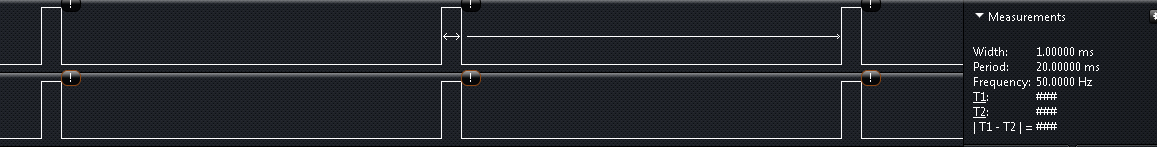
\includegraphics[scale = 0.6]{Screenshots/0_0_Cropped.png}
                \caption{0\degree tilt and 0\degree pan}
            \end{figure}
            \FloatBarrier
            
            \FloatBarrier
            \begin{figure}[htbp]
                \centering
                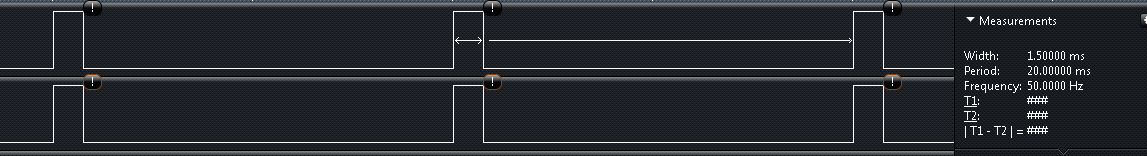
\includegraphics[scale = 0.6]{Screenshots/60_180_Cropped.png}
                \caption{60\degree tilt and 180\degree pan}
            \end{figure}
            \FloatBarrier
            
            \FloatBarrier
            \begin{figure}[htbp]
                \centering
                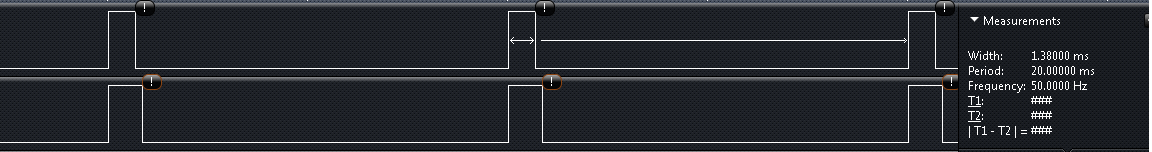
\includegraphics[scale = 0.6]{Screenshots/45_270_Cropped.png}
                \caption{45\degree tilt and 270\degree pan}
            \end{figure}
            \FloatBarrier
        
        \subsection{XBee}
            \textbf{Note}: The pan and tilt angles are reversed in the XBee packets. The pan angle precedes the tilt angle.
            \FloatBarrier
            \begin{figure}[h!]
                \centering
                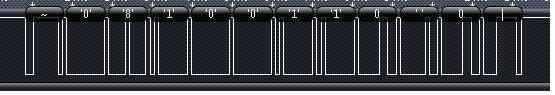
\includegraphics[scale = 1.2]{Screenshots/0_0_XBee_Cropped.png}
                \caption{0\degree tilt and 0\degree pan}
            \end{figure}
            \FloatBarrier
            
            \FloatBarrier
            \begin{figure}[htbp]
                \centering
                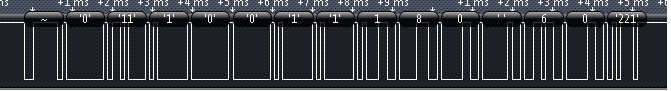
\includegraphics[scale = 1]{Screenshots/60_180_XBee_Cropped.png}
                \caption{60\degree tilt and 180\degree pan}
            \end{figure}
            \FloatBarrier
            
            \FloatBarrier
            \begin{figure}[htbp]
                \centering
                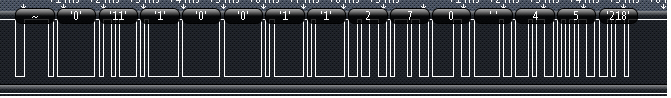
\includegraphics[scale = 1]{Screenshots/45_270_XBee_Cropped.png}
                \caption{45\degree tilt and 270\degree pan}
            \end{figure}
            \FloatBarrier
    
    \section{Difficulties}
        \subsection{Part I}
            The main difficulty for part I was to find a sufficient mathematical calculation that would give us a 1.5ms pulse width and a frequency of 50Hz. Not fully understanding all of the functions provided in the pwmgen code also led to frustration. 
        \subsection{Part II}
            The main difficulty for part II was to find an Algorithm to convert angles into the correct PMW pulse width.
        \subsection{Part III}
            There was a major XBee problem introduced in this lab that wasn't present in Lab3. There was a delay between the LM3S2110 XBee and the actual LM3S2110. The delay caused us to think about what was really going on in the lower level and change our code accordingly. Allowing arrow buttons to change the angles of the servo was also a major problem. We had to increment/decrement the angles everytime an arrow button was pressed. To do this, we had to keep track of the previous angles that were sent to the LM3S2110 and manipulate those angles accordingly. To allow continuous movement of the servo as an arrow button is held, we would needed to change a fundamental part of our code that parsed IR signals. Doing so may drastically change the expectation of our code. We did not want to deal with this problem, so we did not implement this feature.

    
    \newpage
    \appendix
    \section{Code for Lab4}
        \subsection{LM3S2110}
            \lstinputlisting{Code/Lab4_2110.c}
        
        \newpage
        \subsection{LM3S8962}
            \lstinputlisting{Code/Lab4_8962.c}

\end{document}

